%\PassOptionsToPackage{english}{babel}

\documentclass[
	openany,
	% -- opções da classe memoir --
	12pt,				% tamanho da fonte
   % openright,
	%twoside,
    oneside,
    % para impressão em verso e anverso. Oposto a oneside
	a4paper,			% tamanho do papel. 
	english,
	brazil				% o último idioma é o principal do documento
	]{abntex2}

% ---
% Pacotes básicos 
% ---

\usepackage[utf8]{inputenc}		% Codificacao do documento (conversão automática dos acentos)
\usepackage{indentfirst}		% Indenta o primeiro parágrafo de cada seção.
\usepackage{color}				% Controle das cores
\usepackage{graphicx}			% Inclusão de gráficos
\usepackage{microtype} 			% para melhorias de justificação
\usepackage{multicol}			% multiplas colunas no texto
\usepackage{subcaption}
\usepackage{caption}
\usepackage{float}
\usepackage{amsmath}
\usepackage{amssymb}
\usepackage{amsthm}
\usepackage{lipsum}
\usepackage{blindtext}
\usepackage{csvsimple}

% ---
% ---
% Pacotes de citações
% ---
\usepackage[brazilian]{backref}	 % Paginas com as citações na bibl
\usepackage[num]{abntex2cite}	% Citações padrão ABNT

% --- 
% CONFIGURAÇÕES DE PACOTES
% --- 

% ---
% Configurações do pacote backref
% Usado sem a opção hyperpageref de backref
\renewcommand{\backrefpagesname}{Citado na(s) página(s):~}
% Texto padrão antes do número das páginas
\renewcommand{\backref}{}
% Define os textos da citação
\renewcommand*{\backrefalt}[4]{
	\ifcase #1 %
		Nenhuma citação no texto.%
	\or
		Citado na página #2.%
	\else
		Citado #1 vezes nas páginas #2.%
	\fi}%
% ---

% ---
% Informações de dados para CAPA e FOLHA DE ROSTO
% ---
\titulo{Aprendizado profundo com capacidade computacional reduzida: uma aplicação à quebra de captchas.}
\autor{Diogo Felipe Félix de Melo}
\local{Recife}
\data{2015}
\orientador{Pablo de Azevedo Sampaio}



\instituicao{%
	Universidade Federal Rural de Pernambuco -- UFRPE
  	\par
  	Departamento de Computação
    \par
	Bacharelado em Ciências da Camputação
}

\tipotrabalho{Trabalho de Conclusão de Curso}
% O preambulo deve conter o tipo do trabalho, o objetivo, 
% o nome da instituição e a área de concentração 
\preambulo{Monografia apresentada ao Curso de Bacharelado em Ciências da Camputação da Universidade Federal Rural de Pernambuco, como requisito parcial para obtenção do título de Bacharel em Ciências da Camputação.}
% ---


% ---
% Configurações de aparência do PDF final

% alterando o aspecto da cor azul
\definecolor{blue}{RGB}{41,5,195}

% informações do PDF
\makeatletter
\hypersetup{
     	%pagebackref=true,
		pdftitle={\@title}, 
		pdfauthor={\@author},
    	pdfsubject={\imprimirpreambulo},
	    pdfcreator={LaTeX with abnTeX2},
		colorlinks=true,       		% false: boxed links; true: colored links
    	linkcolor=blue,          	% color of internal links
    	citecolor=blue,        		% color of links to bibliography
    	filecolor=magenta,      		% color of file links
		urlcolor=blue,
		bookmarksdepth=4
}
\makeatother
% --- 

% --- 
% Espaçamentos entre linhas e parágrafos 
% --- 

% O tamanho do parágrafo é dado por:
\setlength{\parindent}{1.3cm}

% Controle do espaçamento entre um parágrafo e outro:
\setlength{\parskip}{0.2cm}  % tente também \onelineskip

% ---
% compila o indice
% ---
\makeindex
% ---

% ----
% Início do documento
% ----
\begin{document}

% Seleciona o idioma do documento (conforme pacotes do babel)
%\selectlanguage{english}
\selectlanguage{brazil}

% Retira espaço extra obsoleto entre as frases.
\frenchspacing 

% ----------------------------------------------------------
% ELEMENTOS PRÉ-TEXTUAIS
% ----------------------------------------------------------
% \pretextual
%\begin{figure}[h]
%\centering % este comando é usado para centralizar a figura
%
\includegraphics[width=7cm]{figuras/logo_ufrpe_horizontal.png}\\
%\end{figure}

% \begin{figure}[ht]
% \centering
% \begin{minipage}[b]{0.45\textwidth}
% 
\includegraphics[height=3cm]{figuras/logo_ufrpe_horizontal.png}
% \end{minipage}
% \qquad
% \begin{minipage}[b]{0.45\textwidth}
% 
\includegraphics[height=2.5cm]{figuras/logo_bsi.pdf}
% \end{minipage}
% \end{figure}

%\begin{minipage}[t]{1\textwidth}
	\begin{figure}[ht]
		
\includegraphics[height=3cm]{figuras/logo_ufrpe_horizontal.png}
		\hspace{5.5cm}
    	
\includegraphics[height=3cm]{figuras/bcc_logo.png}
	\end{figure}    
%\end{minipage}

% ---
% Capa
% ---
\imprimircapa
% ---
% ---
% Folha de rosto
% (o * indica que haverá a ficha bibliográfica)
% ---
\imprimirfolhaderosto
% ---

% dedicatoria
%\begin{dedicatoria}
   \vspace*{\fill}
   \centering
   \noindent
   \textit{À \ldots\\} \vspace*{\fill}
\end{dedicatoria}

% agradecimentos
\begin{agradecimentos}

Meus pais, familiares e amigos.

Ao meu orientador, por toda a paciência e dedicação. 

\end{agradecimentos}

% epigrafe
%\begin{epigrafe}
    \vspace*{\fill}
	\begin{flushright}
		\textit{``A persistência é o caminho do êxito.'' \\
		(Charles Chaplin)}
	\end{flushright}
\end{epigrafe}

% resumo e abstract
\setlength{\absparsep}{18pt} % ajusta o espaçamento dos parágrafos do resumo
\begin{resumo}
 



 \textbf{Palavras-chave}: Aprendizado de Maquina, Aprendizado Profundo, CAPTCHA.
\end{resumo}


%\begin{resumo}[Abstract]
 \begin{otherlanguage*}{english}
  
During the last decade, Deep Neural Networks has been shown to be a powerfull machine learn technique. Generally, to obtain relevant results, these techniques require high computacional power and large volumes of data. Neverthless, a careful project of trainig and archtecture may help to reduce these requirements. In the this work we present a comparative approach to the application of deep neural networks to text based CAPTCHAs. We studied models that are capable of learn to segment and identify the text content of images, only based on examples. By experimentation of different hiper-parameters and architectures, we were capable to obtain a final model with $96.06\%$ of token prediction accuracy in approximately 3 hours of training in a simple personal computer.
 
   \vspace{\onelineskip}
 
   \noindent
   \textbf{Keywords}: Machine Learning, Deep Learning, CAPTCHA.
 \end{otherlanguage*}
\end{resumo}

% ---
% inserir lista de ilustrações
% ---
\pdfbookmark[0]{\listfigurename}{lof}
\listoffigures
\cleardoublepage
% ---

% ---
% inserir lista de tabelas
% ---
\pdfbookmark[0]{\listtablename}{lot}
\listoftables*
\cleardoublepage
% ---

% ---
% inserir lista de abreviaturas e siglas
% ---
\begin{siglas}
  \item[CAPTCHA] Completely
Automated  Public  Turing  tests  to  tell Computers  and
Humans ApartUser Datagram Protocol
  \item[OCR] Optical Character Recognition

\end{siglas}
% ---

% ---
% inserir o sumario
% ---
\pdfbookmark[0]{\contentsname}{toc}
\tableofcontents*
\cleardoublepage
% ---



% ----------------------------------------------------------
% ELEMENTOS TEXTUAIS
% ----------------------------------------------------------
\textual

% ----------------------------------------------------------
% inclusao das secoes do texto
% ----------------------------------------------------------
\chapter{Introdução}

Algoritmos de aprendizado baseados em neurologia são conhecidos desde meados do século passado \cite{perceptron_58}. Das proposições iniciais até os dias de hoje, essa classe de modelos tem evoluído em complexidade e técnicas de forma contínua,
culminando em um alto poder de expressividade e níveis cada vez mais abstratos de representação (ver \cite{Goodfellow-et-al-2016} ou \cite{jurgenReview2015} para uma breve revisão histórica). Os poucos resultados teóricos disponíveis demonstram que redes neurais possuem um alto poder de generalização, sendo capazes de, sob certas circunstâncias, codificar diversas classes de funções \cite{Barron1993UniversalAB, Andoni2014PolyAprox}. Apesar dos avanços na área, foi apenas recentemente que modelos neurais começaram a redefinir o estado da arte, superando outras classes de algoritmos de aprendizado de máquina \cite{imagenet_2012} e até mesmo alcançando performances sobre-humanas \cite{mnih2015humanlevel}. Á estes modelos propostos mais recentemente é comum a denominação de redes neurais de aprendizado profundo. Tais avanços foram possíveis devido a três fatores chaves: a viabilização de bases de dados cada vez maiores, o aumento do poder computacional e o desenvolvimento de novas arquiteturas e técnicas de treino.

A crescente melhoria de performance dos modelos neurais de aprendizado profundo tem motivado estudos em áreas onde é preciso distinguir computadores e humanos. Dentre essas áreas temos os CAPTCHAs \cite{captcha2003} (do inglês Completely Automated  Public  Turing  tests  to  tell  Computers  and Humans Apart) ou HIPs \cite{lectures2005HIP} (do inglês Human Interaction Proofs), que definem uma coleção de técnicas que tem como objetivo bloquear a ação de agentes autônomos na rede mundial de computadores. Um dos subconjuntos mais conhecidos dessas técnicas talvez seja o de CAPTCHAs baseados em texto \cite{captcha_review_2017}. Nesse tipo de desafio, uma imagem contendo uma sequência de caracteres é exibida e a validação é feita pela comparação entre o texto informado pelo usuário e a resposta correta. Formulado como um problema de aprendizado de máquina, desejamos descobrir de forma automatizada um mapa entre a imagem e o texto codificado. Na versão informada do problema, um ser humano escolhe previamente técnicas de preprocessamento (filtros, segmentação de caracteres, etc.) antes que o aprendizado propriamente dito ocorra. Ajudados por humanos, redes neurais simples e com poucos exemplos conseguem resultados satisfatórios nesse tipo de desafio \cite{lectures2005HIP}. De fato, mesmo técnicas ingênuas como contagem de \textit{pixels} podem obter bons resultados quando o preprocessamento correto é fornecido \cite{naivecaptcha}. Na versão não informada, entretanto, encontrar mapas imagem-texto de forma automatizada é usualmente muito mais desafiador. Em trabalhos recentes, foram relatados modelos baseados em redes neurais capazes de burlar esse tipo de desafio com acurácias de acerto próximos à humana em sequências sorteadas a partir de um repositório \cite{captcha_break_2013} e modelos com alta eficiência de dados \cite{captcha_break_2017}. Para o problema geral de quebrar CAPTCHAs baseados em texto, entretanto, modelos de aprendizado profundo ainda mostram desempenho inferior ao humano. Contudo, pesquisas recentes apontam para avanços claros nos próximos anos \cite{Bursztein2014TheEI}. Em comum, esses modelos possuem a necessidade de \textit{clusters} e/ou sistemas de computação sob demanda para treinamento, com hardware de alto poder de processamento e/ou paralelização, como GPUs e TPUs. Adicionalmente, as bases de treinamento necessárias comumente alcançam alguns terabytes e envolvem grandes operações de aquisição e/ou geração.

Neste trabalho propomos uma abordagem comparativa entre diferentes arquiteturas de redes neurais para a solução de CAPTCHAs baseados em texto sem informação humana, nos restringindo, entretanto, à um ambiente com poder computacional reduzido. Pretendemos mostrar que é possível fazer uso dessas técnicas em um mero computador pessoal (na contramão dos trabalhos usualmente encontrados na literatura) e ainda obter resultados próximos ao estado da arte. Este trabalho se encontra organizado como segue. No capítulo \ref{cap:captchas} apresentamos uma breve introdução à diferentes tipos de CAPTCHAs, com ênfase em desafios baseados em texto. Sequencialmente, no capítulo \ref{cap:neurais}, arquiteturas e técnicas de projeto e treino de redes neurais comuns na literatura são abordados, os principais resultados do uso dessas técnicas em CAPTCHAs de texto explorados e nossas considerações iniciais sobre essa aplicação apresentadas. No capítulo \ref{cap:modelagem} uma descrição das arquiteturas dos modelos usados neste estudo é feita em conjunto com uma breve fundamentação para as escolhas. No capítulo \ref{cap:metodologia}, detalhes dos experimentos realizados são formalizados. Por fim, no capítulo \ref{cap:resultados} os resultados dos experimentos são apresentados e analisados e no capítulo \ref{cap:concusao} nossas conclusões e considerações finais apresentadas.

\chapter{Fundamentação}

\section{CAPTCHAS}

CAPTCHAS podem ser formulados com um desafio sobre um conjunto de domínio cuja a resposta é um token. O domínio pode ser um trecho de áudio, uma sequencia de imagens ou até mesmo o histórico de navegação ou ambiente de desafiado. O token pode ser constituído de um conjunto de ações, o texto extraído do áudio ou imagem, ou possuir um histórico de navegação de baixo risco.

CAPTCHAS de texto podem ser vistos como um problema de extração de texto em imagens, sendo assim uma generalização para o problema de OCR (optical character recognition). Entretanto, CAPTCHAS são especialmente desenvolvidos para serem de difícil solução para computadores e preferencialmente fáceis para seres humanos. Assim, algoritmos usuais de OCR tendem a demonstrar baixo desempenho na solução desses desafios.



\section{Redes Neurais}

De forma geral, aprendizado de máquina supervisionado pode ser descrito como, dado um conjunto de exemplos $D = \{(x, y)\}$, onde $x$  pertence ao domínio do treino e $y$ o rótulo associado, desejamos encontrar a função $\hat{y} = f(x)$, de tal modo que $\hat{y}$ seja o mais similar o possível à $y$ dado $x$. Por 'mais similar o possível' entende-se que conhecemos uma função de erro que é tão menor quanto melhor for a aproximação dada por $f(x)$. Formalmente, desejamos encontrar $f^*$ tal que
\begin{equation}
f^* = \min_f \langle err(y, f(x)) \rangle_{D},
\end{equation}   
onde $\langle \ldots \rangle_{D}$ representa o valor esperado no conjunto $D$. $J_D = \langle err(y, f(x)) \rangle_{D}$ é usualmente referido como o \textit{custo}.

Redes neurais são um conjunto de técnicas inspiradas em processos cognitivos desempenhados pelo sistema nervoso que fornecem uma maneira de descrever famílias de funções. Dada uma família de funções $f^{\Theta} : x \leftarrow y$ definida por uma rede neural e parametrizadas por $\Theta$, podemos vasculhar o espaço de busca induzido por $\{\Theta\}$ para encontrar um função que satisfaça alguma propriedade de interesse. Em particular, no caso de aprendizado de máquina, estamos interessados em encontrar o parâmetro $\Theta^*$ tal que:
\begin{equation}
\Theta^* = \min_{\Theta} \langle err(y, f^{\Theta}(x)) \rangle_{D}.
\end{equation} 




Quando munidos de um algoritmo de busca, podemos vasculhar a família de funções descritas por uma rede neural em 

Redes Neurais 



Camadas Totalmente conectadas. 






\chapter{Modelagem}\label{modelagem}



definição das redes
definição da nomenclatura
 

\chapter{Metodologia}

\section{Geração dos CAPTCHAS}

foram geradas 30000 imagens usando diferentes efeitos e cores com tokens de comprimento fixo em 5 utilizando-se a biblioteca \cite{simplecaptcha}

um exemplo constitui de um tensor $(200, 50, 3)$ e de um token $(5, 36)$

exemplos normalizados entre 0-1, token codificado one-hot, de modo que 

\begin{equation}
   p(y[i]|x)= 
	\begin{cases}
		1,	& \text{if } y[i]=w_i\\
		0,  & \text{caso contrário.}
	\end{cases}
\end{equation}

Os 30000 exemplos foram separados, de forma aleatória, em dois conjuntos:
o conjunto de treino, $D_{tr}$, e o de validação, $D_{va}$, com 20000 e 10000 exemplos, respectivamente.

\begin{figure}[ht]
	\begin{subfigure}{.5\textwidth}
		\centering
	 	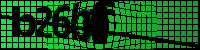
\includegraphics[width=.9\linewidth]{figuras/7103_b26bf.png}
		\caption{b26bf}
	\end{subfigure}
	\begin{subfigure}{.5\textwidth}
		\centering
		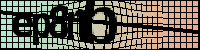
\includegraphics[width=.9\linewidth]{figuras/9456_ep8nb.png}
		\caption{ep8nb}
	\end{subfigure}%
	\vspace{.05\linewidth}

	\begin{subfigure}{.5\textwidth}
		\centering
		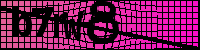
\includegraphics[width=.9\linewidth]{figuras/21856_b7rw8.png}
		\caption{b7rw8}
	\end{subfigure}
	\begin{subfigure}{.5\textwidth}
		\centering
		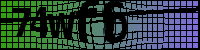
\includegraphics[width=.9\linewidth]{figuras/19816_74wf6.png}
		\caption{74wf6}
	\end{subfigure}%
	\vspace{.05\linewidth}

	\begin{subfigure}{.5\textwidth}
		\centering
		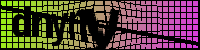
\includegraphics[width=.9\linewidth]{figuras/12248_dnyny.png}
		\caption{dnyny}
	\end{subfigure}
	\begin{subfigure}{.5\textwidth}
		\centering
		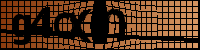
\includegraphics[width=.9\linewidth]{figuras/8873_g4cxh.png}
		\caption{g4cxh}
	\end{subfigure}%
	\vspace{.05\linewidth}

	\caption{Exemplos de CAPTCHAS gerados e seus respectivos tokens.}
\end{figure}



\section{Grandezas de interesse}

\begin{equation}
	S_i^{(D)} = \sum_{(x,y) \in D} p(y[i]|x) \log \hat{p}(y[i]|x)
\end{equation}

\begin{equation}
	acc_w^{(D)} = \frac{N_w}{|D|}
\end{equation}

\begin{equation}
\hat{p}_i^{(D)} = acc_i^{(D)} = \frac{N_i}{|D|}
\end{equation}

\begin{equation}
\hat{p_w}^{(D)} = \prod_{i} \hat{p}_i^{(D)}
\end{equation}

\begin{equation}
loss_i^{(D)} = \frac{S_i}{|D|}
\end{equation}

\begin{equation}
loss^{(D)} = \sum_{i} loss_i^{(D)}
\end{equation}

$t$ tempo total de execução de uma época (treino + validação)
$\tilde{t}$ tempo de treino em uma época.

\section{Treino e Validação}

Todos as redes foram treinadas em um mesmo computador com pentium core i5, 8gb de ram usando tensorflow.

Redes inicializadas segundo critério de \cite{xavier_init}

etapa de treino consiste em
mini batch: sortear $D_{batch} \subset  D_{tr}$, com $|D_{batch}| = 10$ e minimizar  $S_i$'s nesse conjunto usando com \cite{adam_op} com taxa de aprendizado $l_r$. 

O treino em uma época consiste em repetir $|D_{tr}|/|D_{batch}|$ vezes.

calcular as grandezas de interesse em $D_{tr}$ e $D_{va}$


experimentos realizados com diferentes taxas de aprendizado durante 10 épocas. Limite superior e inferior escolhidos manualmente baseados em melhor desempenho aprendizado rápido para a superior e estável para a inferior. Decaimento linear.

Treinado usando critério de parada: mínimo de 10 épocas, máximo de 50 épocas, custo no conjunto de validação na época atual não maior que o .10 do menor valor encontrado até agora, custo no conjunto de treinamento atual menor que .03 da média dos últimos 5 valores. Inspirado em \cite{lutz_early_stop}

\chapter{Resultados} \label{resultados}




\cite{otaro}
5x5 k64, 5x5 e 128, 5x5 e 256, 3x3k512, 16896x4096 dense, 5 camadas densas 4096x36. alcança 76,6 no teste, 95,3 no treino



% ----------------------------------------------------------
% ELEMENTOS PÓS-TEXTUAIS
% ----------------------------------------------------------
\postextual
% ----------------------------------------------------------

% ----------------------------------------------------------
% Referências bibliográficas
% ----------------------------------------------------------
\bibliography{referencias.bib}


%---------------------------------------------------------------------
% INDICE REMISSIVO
%---------------------------------------------------------------------
\phantompart
\printindex
%---------------------------------------------------------------------

\end{document}
